\documentclass[handout]{beamer}
\usepackage[utf8]{inputenc}
\usepackage{graphics}
\mode<presentation> {
	\usetheme{unc}}
\setbeamertemplate{navigation symbols}{} % To remove the navigation symbols from the bottom of all slides uncomment this line

\usepackage{graphicx} % Allows including images
\usepackage{booktabs} % Allows the use of \toprule, \midrule and \bottomrule in tables


\usepackage{hyperref}
\hypersetup{linkcolor=blue,colorlinks=true}


% Remove symbols
\beamertemplatenavigationsymbolsempty


%\usetheme{default}

\usefonttheme{serif}

%----------------------------------------------------------------------------------------
%	TITLE PAGE
%----------------------------------------------------------------------------------------


\title[UNC Conflict Research]{\LARGE{UNC Conflict Research and Ukraine-Russia War Overview}}
\author[POLI 150]{Steven Saroka}
\institute{POLI 150}
\date{6 July 2023}


\begin{document}
	
	\begin{frame}
		\titlepage % Print the title page as the first slide
	\end{frame}
	
	
	%----------------------------------------------------------------------------------------
	%	PRESENTATION SLIDES
	%----------------------------------------------------------------------------------------
	
	%% Slide outline
	
	\begin{frame} 
		\frametitle{\LARGE{Today's Class}}
		\begin{itemize}
			\Large{
				\item UNC Conflict Research
				\\~\\
				\item Overview of Ukraine-Russia War
				\\~\\ 
				\item Theory application}
		\end{itemize}
	\end{frame}
	
\begin{frame} 
	\frametitle{\LARGE{Central Question}}
	\centering
	\Large{What conflict research has been published recently at UNC? How can we apply class concepts to the Russia-Ukraine war?}
\end{frame}

\begin{frame} 
	\frametitle{\LARGE{Key Terms}}
	\begin{itemize}
		\item Market power politics
		\item Strategic delay
		\item Grey zone tactics
		\item Salami expansion
		\item Petrodollar system
	\end{itemize}
\end{frame}

\begin{frame} 
	\frametitle{\LARGE{Gent and Crescenzi Review}}
	Group yourselves and answer the following:
	\begin{itemize}
		\item What was their main point?
		\item Why might states want to expand their territorial reach?
		\item What can prevent them from doing so?
		\item What strategies can states pursue to expand their territorial reach and market power?
	\end{itemize}
\end{frame}

\begin{frame} 
	\frametitle{\LARGE{Market Power Politics}}
	\begin{itemize}
		\item This chapter (and the rest of the book) is concerned with how and when states engage in territorial expansionist behaviors. \pause
		\item \textbf{Market power politics theory argues that competition for market power gives states incentives to expand their territory or prevent other states from expanding.}
		\item However, since WWII, a norm of international respect for settled borders has (generally) prevailed. \pause
		\item This may lead to constraints on a state's actions. 
	\end{itemize}
\end{frame}

\begin{frame} 
	\frametitle{\LARGE{Constraints}}
	\begin{itemize}
		\item If a state's goal is to expand its market power by expanding its territorial control, what might constrain its actions? Two factors: \pause
		\item \textbf{Economic interdependence}: sufficient dependence on a globalized economy, which would be disrupted by open conflict, can dissuade states from open conflict. \pause
		\item \textbf{International institutions}: states may anticipate that the dispute resolution mechanisms would lead to an outcome that would be suboptimal from a domestic political standpoint.
	\end{itemize}
\end{frame}	

\begin{frame} 
	\frametitle{\LARGE{Constraints}}
	\begin{itemize}
		\item In situations of extremely low constraints, states may simply go to war to grab economically desirable territory. \pause
		\item In situations of extremely high constraints, states will be forced to accept peaceful settlements, even if they are suboptimal. \pause
		\item This theory is most concerned with situations where there is a mixture of high and low constraints. \pause 
		\item In these cases, states can use a tactic of \textbf{strategic delay}.
	\end{itemize}
\end{frame}	

\begin{frame} 
	\frametitle{\LARGE{Strategic Delay}}
	\begin{itemize}
		\item \textbf{Strategic delay}: purposeful postponement of a violent or non-violent settlement of a dispute  with the goal of trying to achieve a more preferable outcome in the future. \pause
		\item This delaying tactic gives states time to implement \textbf{gray zone tactics}: not the overt use of lethal  force by a military, but not also behavior traditionally accepted within international diplomacy. \pause
		\begin{itemize}
			\item These tactics let states slowly pursue their territorial claims over time, while avoiding major armed conflict. \pause
		\end{itemize}	
		\item Grey zone tactics frequently involve \textbf{salami expansion}: small, cumulative steps each of which is too minor to fight over, but at their culmination leads to an outcome that would have triggered conflict if carried out all at once. 
	\end{itemize}
\end{frame}

\begin{frame} 
	\frametitle{\LARGE{The End Goal}}
	\begin{itemize}
		\item The overarching goal of states engaging in this behavior is to use this expanded territorial control to increase a state's \textbf{market power}, allowing it to extract higher profits (``rents"), especially if an industry is state-controlled. \pause
		\item This is desirable for several reasons:
		\begin{itemize}
			\item Increased state revenue
			\item Domestic political stability (if resource is vital for daily life)
			\item International bargaining power
		\end{itemize}
		\item This theory focuses on ``hard commodities," which are natural resoures like oil, gas, or rare minerals.	
	\end{itemize}
\end{frame}

\begin{frame} 
	\frametitle{\LARGE{Bapat Review}}
	Group yourselves and answer the following:
	\begin{itemize}
		\item What was his main point?
		\item What is the relationship between the host state and the US?
		\item What is the relationship between the host state and the terrorists?
		\item What effect does US military aid have on terrorism?
	\end{itemize}
\end{frame}

\begin{frame} 
	\frametitle{\LARGE{Petrodollar System}}
	\begin{itemize}
		\item \textbf{Petrodollar system}: the sale of petroleum in US dollars. \pause
		\item The majority of petroleum and related products are sold in USD. \pause
		\item Why? One consequence of the US going off the gold standard in the 1970s. 
	\end{itemize}
\end{frame}

\begin{frame} 
	\frametitle{\LARGE{Formal Model}}
	\begin{itemize}
		\item If the host state is participating in the petrodollar system by producing and exporting oil, this helps America's economy by keeping the dollar valuable. \pause
		\item Given the economic benefits of a strong dollar, this means the US has rational incentives to protect such an economic system. \pause
		\item This can involve the US sending military aid to oil producers (``host states") to ensure their security, as a destabilized or failed state will no longer participate in the global petrodollar system.
	\end{itemize}
\end{frame}

\begin{frame} 
	\frametitle{\LARGE{Formal Model: Moral Hazards}}
	\begin{itemize}
		\item Say that host state has a terrorist problem. \pause
		\item If it receives military aid to increase its security, this decreases its incentives to bargain with or eliminate the terrorists. Why? \pause
		\begin{itemize}
			\item \textbf{If the terrorism stops, so does the flow of aid.}
		\end{itemize}
		\item This aid strengthens the government such that its leaders are able to stay in power (particularistic benefits), while the costs of an ongoing terrorism campaign are borne by the general population.
	\end{itemize}
\end{frame}

\begin{frame} 
	\frametitle{\LARGE{Formal Model: Moral Hazards}}
	\begin{itemize}
		\item This incentive structure is especially helpful to the host state if it is engaging in the kinds of corruption and human rights abuses that normally lead to aid being suspended. \pause
		\item In response to any threatened decrease in aid, the host state can argue that it is in America's economic interest to keep the state functional, as this way its participation in the petrodollar system continues. 
	\end{itemize}
\end{frame}

\begin{frame} 
	\frametitle{\LARGE{Formal Model: The Take-Away}}
	\begin{itemize}
		\item US military aid for fighting terrorism does not actually decrease the amount of terrorism, but instead prolongs it, while also serving US interests in stability of the petrodollar system.
	\end{itemize}
\end{frame}

% pic from https://www.thehindu.com/news/international/ukraine-russia-crisis-live-updates-march-29-2022/article65269704.ece
% description: Ukrainian soldiers watch debris from a Russian tank after recent fights in the town of Trostsyanets, some 400km (250 miles) east of capital Kyiv, Ukraine, on March 28, 2022. | Photo Credit: AP 
\begin{frame} 
	\frametitle{\LARGE{Ukraine-Russia War}}
	\begin{figure}[ht!]
		\centering
		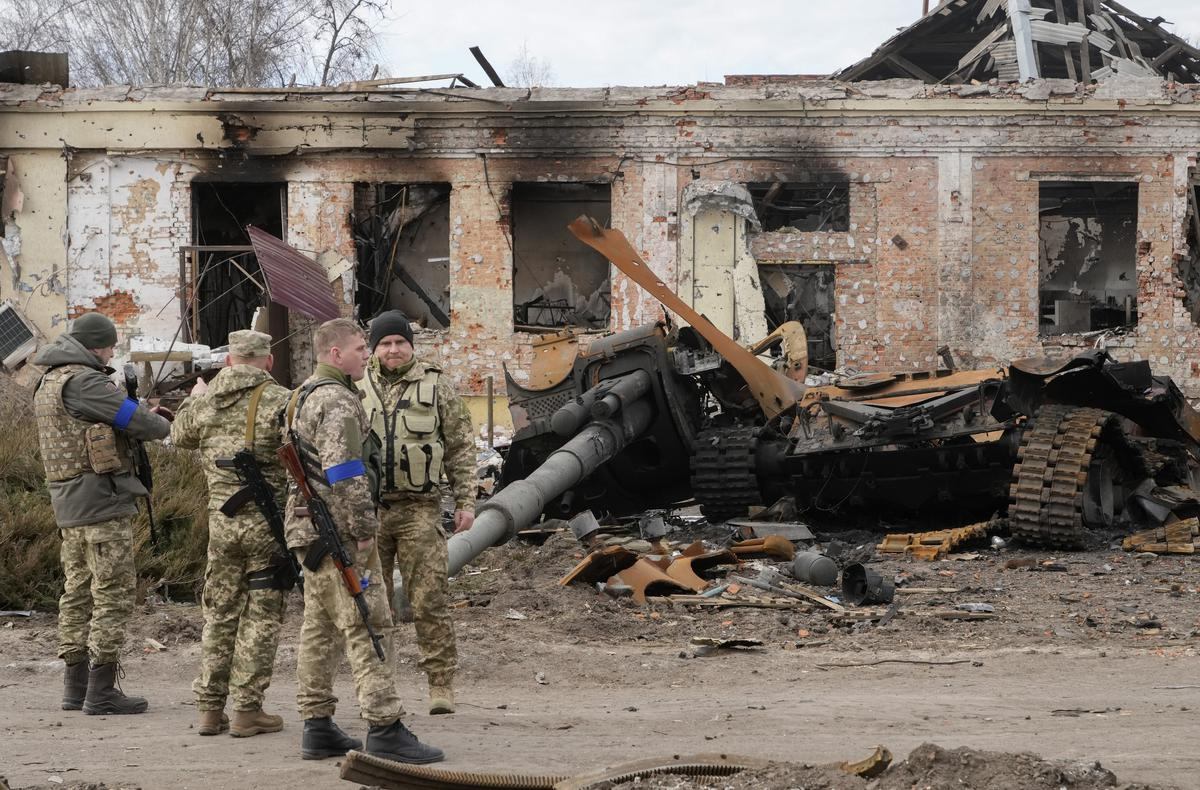
\includegraphics[width=\textwidth,height=0.9\textheight,keepaspectratio]{Russia_Ukraine_War_33204.jpg-795e2.jpg}
	\end{figure}
\end{frame}

%info pulled from NYT writeup and wikipedia
\begin{frame} 
	\frametitle{\LARGE{Ukraine Pre-War Crisis Basic Timeline}}
	\begin{itemize}
		\item 2014: Ukraine's pro-Russian government is ousted by popular protest. \pause
		\item Their replacements are more friendly towards the West than towards Putin's Russia. \pause
		\item Russia responds by annexing Crimea, a part of Ukraine, before backing separatists within two regions of eastern Ukraine in their bid to violently secede from Ukraine. \pause
		\item US and allies imposed sanctions on Russia in retaliation.
		\item This creates a low-level conflict that continued until late February 2022, with tensions rising as Russian troops massed on the border.	
		\item Russia invades on February 24, 2022.
	\end{itemize}
\end{frame}

\begin{frame} 
	\frametitle{\LARGE{Basic Map 1: Pre-War Boundaries}}
	\begin{figure}[ht!]
		\centering
		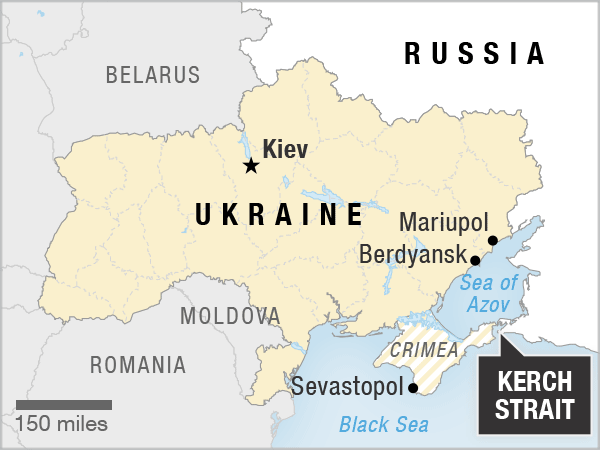
\includegraphics[width=\textwidth,height=0.9\textheight,keepaspectratio]{map1.png}
	\end{figure}
\end{frame}

%https://www.brookings.edu/blog/brookings-now/2015/05/21/10-maps-that-explain-ukraines-struggle-for-independence/
\begin{frame} 
	\frametitle{\LARGE{Basic Map 2: Soviet Bloc}}
	\begin{figure}[ht!]
		\centering
		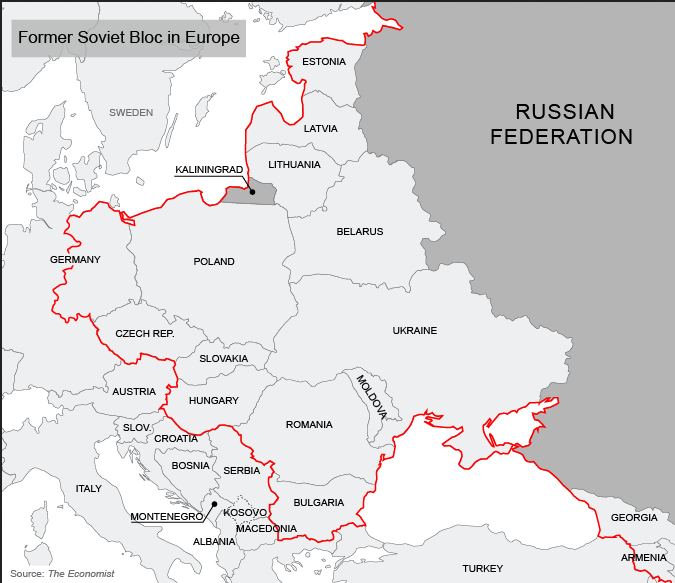
\includegraphics[width=\textwidth,height=0.9\textheight,keepaspectratio]{map2.png}
	\end{figure}
\end{frame}

\begin{frame} 
	\frametitle{\LARGE{Basic Map 3: Russian as Unique Language}}
	\begin{figure}[ht!]
		\centering
		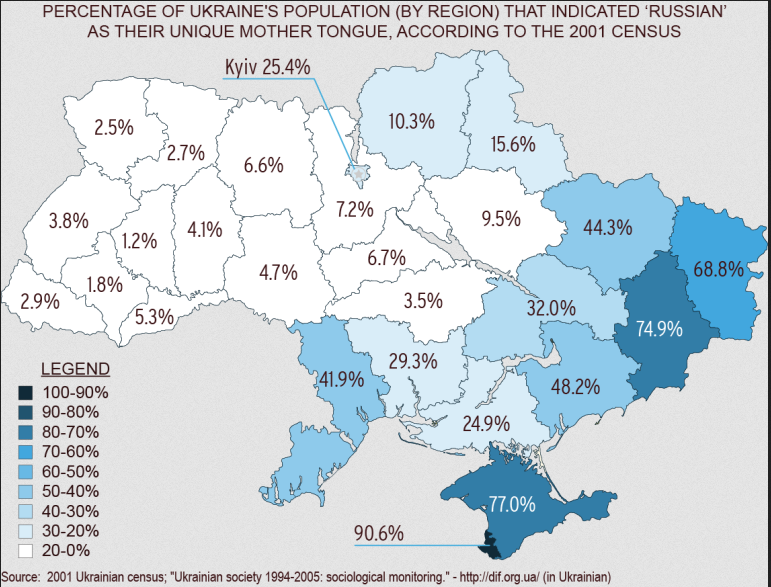
\includegraphics[width=\textwidth,height=0.9\textheight,keepaspectratio]{map3.png}
	\end{figure}
\end{frame}

\begin{frame} 
	\frametitle{\LARGE{Basic Map 4: Russian Unification Poll}}
	\begin{figure}[ht!]
		\centering
		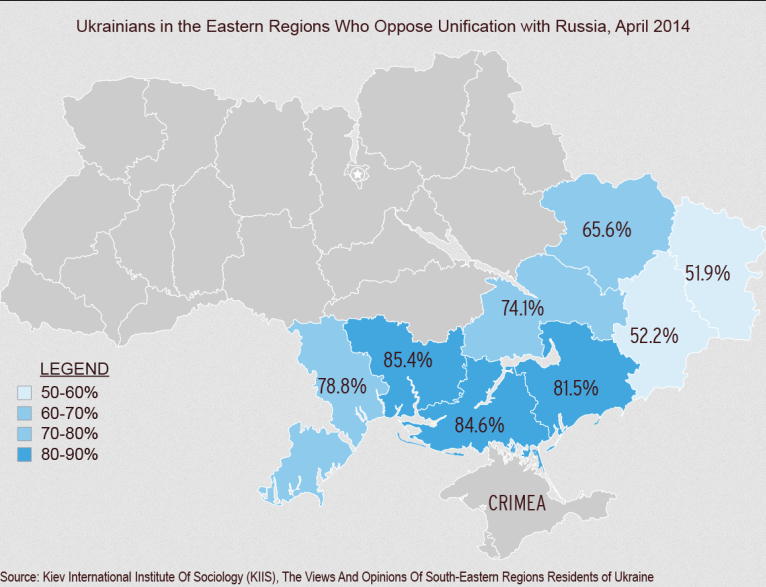
\includegraphics[width=\textwidth,height=0.9\textheight,keepaspectratio]{map4.png}
	\end{figure}
\end{frame}

\begin{frame} 
	\frametitle{\LARGE{What Do These Maps Tell Us?}}
	\begin{itemize}
		\item Ukraine used to be part of the Soviet bloc, only gaining independence after the fall of the Soviet Union. \pause
		\item Russia's Black Sea Fleet was based in Sevastopol (both before and after fall of USSR) by treaty with Ukraine. \pause
		\item Within Ukraine's population, its eastern regions are most likely to both have unique Russian speakers and those who do not oppose some kind of unification with Russia. \pause
		\begin{itemize}
			\item This does not mean that this conflict divides by linguistic lines, as plenty of Ukrainians in the western areas also speak Russian. \pause
			\item Out of the entirety of Ukraine, however, the most likely place for a pro-Russian rebellion would be in the eastern part of the country.
		\end{itemize}
	\end{itemize}
\end{frame}

\begin{frame} 
	\frametitle{\LARGE{Why Does Russia Care?}}
	Why is the Russian state acting this way?
	\begin{itemize}
		\item Indications from public statements that Russia's President Putin considers the fragmentation of the Soviet bloc to be a massive blow to Russia's power and prestige. \pause
		\item Putin appears to be trying to recover the zone of influence Russia had over the Soviet bloc during the days of the USSR. \pause
		\begin{itemize}
			\item This effort would be threatened by a Ukraine that shifted its foreign policy stance to more firmly align with Western Europe, which is exactly what was happening after 2014.
		\end{itemize}
	\end{itemize}
\end{frame}

\begin{frame} 
	\frametitle{\LARGE{Why Does Russia Care?}}
	Why is the Russian state acting this way?
	\begin{itemize}
		\item This effort has led to consistent use of propaganda to portray Crimea and areas of eastern Ukraine as being rightfully Russian, not Ukrainian. \pause
		\item Domestic incentives: Putin may have aimed to trigger a rally effect, as Russia faced a domestic economic downturn and the pandemic. \pause
		\item Finally, Putin appears to see this as a way to stop the spread of NATO's influence. \pause
		\begin{itemize}
			\item Backfired as NATO invited Sweden and Finland to join, while Bosnia and Herzegovina, Georgia, and Ukraine have all declared interest in joining...
		\end{itemize}
	\end{itemize}
\end{frame}

\begin{frame} 
	\frametitle{\LARGE{What about NATO?}}
	What does NATO have to do with any of this?
	\begin{itemize}
		\item Ukraine is \textbf{not} a NATO member state. \pause
		\item However, the last 30 years have seen increasing ties between NATO member states and Ukraine. In particular, their security cooperation has steadily grown. \pause
		\item More recently (2017 onwards), joining NATO is an explicit goal of Ukraine's foreign policy.
		\item Recall NATO's post-Cold War expansion...
	\end{itemize}
\end{frame}

\begin{frame} 
	\frametitle{\LARGE{NATO Global Membership}}
	\begin{figure}[ht!]
		\centering
		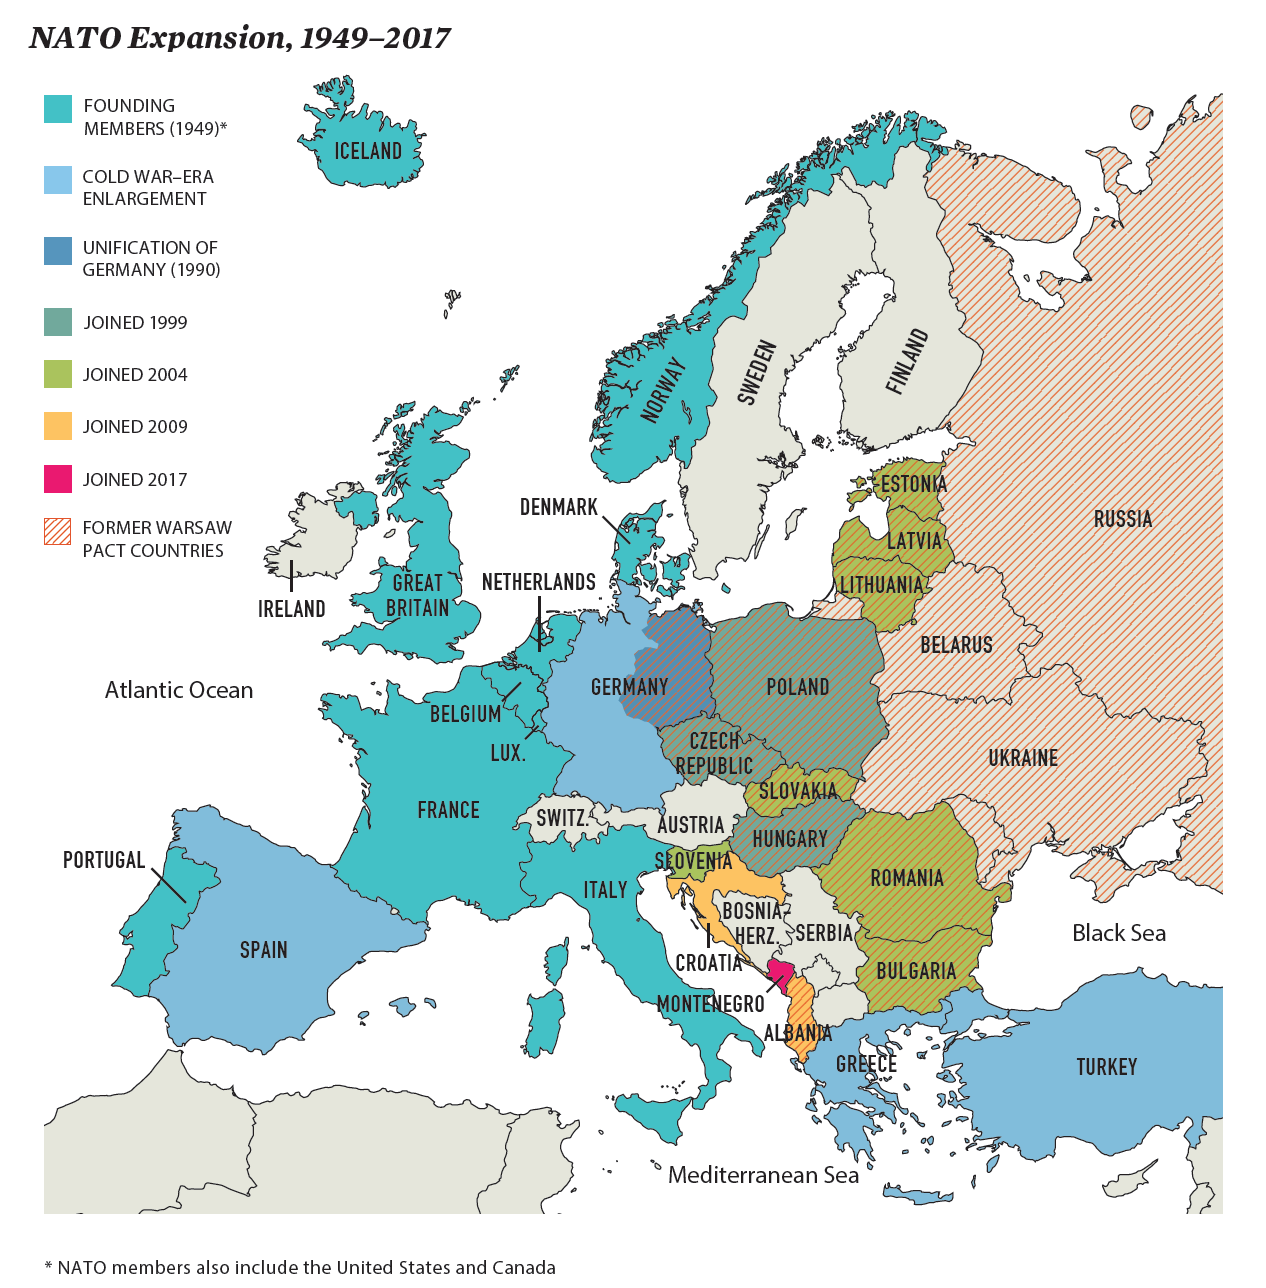
\includegraphics[width=\textwidth,height=\textheight, keepaspectratio]{nato.png}
	\end{figure}
\end{frame}

\begin{frame} 
	\frametitle{\LARGE{What about NATO?}}
	What does NATO have to do with any of this?
	\begin{itemize}
		\item What does this expansion look like? \pause \textbf{Like NATO is encircling Russia.} \pause
		\item In particular, note how it has absorbed several former Warsaw Pact states. \pause
		\item In a realist, security-oriented view of the world, Putin's conclusion that this is an attempt to limit Russian power and influence is not an unreasonable one (setting aside the question of whether it is correct).
	\end{itemize}
\end{frame}

%https://www.washingtonpost.com/world/2022/01/21/ukraine-russia-explain-maps/
%https://ukraine.un.org/sites/default/files/2021-10/Conflict-related%20civilian%20casualties%20as%20of%2030%20September%202021%20%28rev%208%20Oct%202021%29%20EN.pdf
\begin{frame} 
	\frametitle{\LARGE{Low-Level Conflict in Ukraine}}
	From 2014-2022, Russia avoided large-scale direct military confrontation.
	\begin{itemize}
		\item Russia aided the establishment of a small separatist-controlled enclave in eastern Ukraine's Donbass and Luhansk provinces. \pause
		\item Separatists were pro-Russian but not helped by \textit{uniformed} Russian troops at this stage. \pause
		\item From 2014 to the start of open war in February 2022, approximately 14,000 died, of whom about 3,000 were civilians. \pause
		\item Conflict was characterized by many short-lived ceasefires.
	\end{itemize}
\end{frame}

\begin{frame} 
	\frametitle{\LARGE{Separatist Regions}}
	\begin{figure}[ht!]
		\centering
		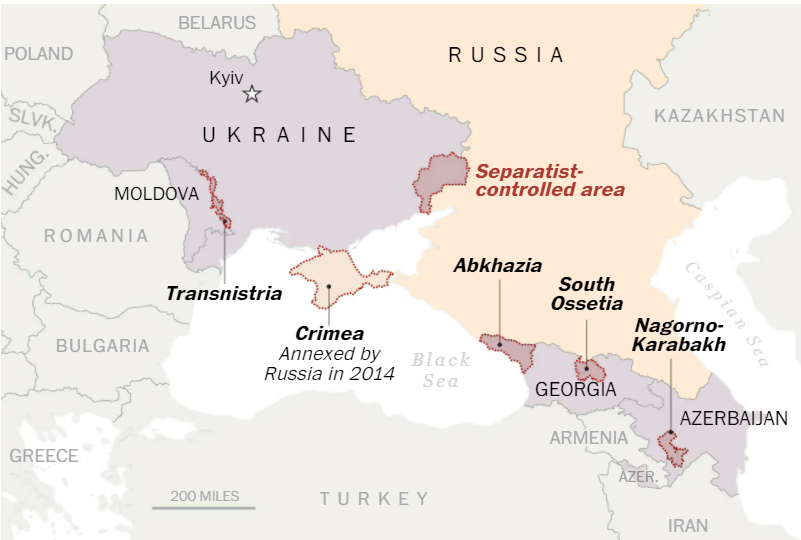
\includegraphics[width=\textwidth,height=\textheight, keepaspectratio]{sep1.png}
	\end{figure}
\end{frame}

\begin{frame} 
	\frametitle{\LARGE{Separatist Regions}}
	\begin{figure}[ht!]
		\centering
		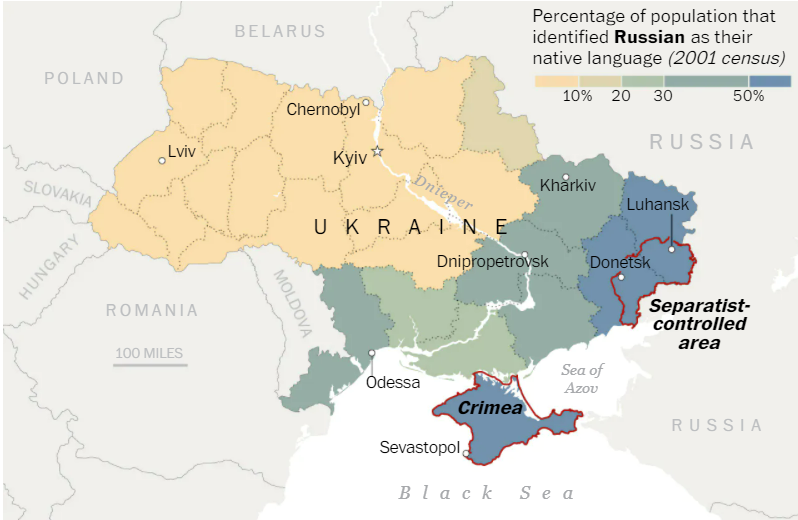
\includegraphics[width=\textwidth,height=\textheight, keepaspectratio]{sep2.png}
	\end{figure}
\end{frame}

%https://www.nytimes.com/article/russia-ukraine-nato-europe.html?name=styln-russia-ukraine&region=TOP_BANNER&block=storyline_menu_recirc&action=click&pgtype=Interactive&variant=0_Control&is_new=false
\begin{frame} 
	\frametitle{\LARGE{Increasing Tension}}
	\begin{itemize}
		\item By late February 2022, 100,000 Russian troops had massed on the border with Ukraine, while Putin made several demands of the West and NATO. \pause
		\item Most notably, he has demanded NATO cease its eastern expansion and never admit Ukraine as a member. \pause
		\item If the US had accepted these demands, it would have been a clear infringement on its sovereignty. \pause
		\item Meanwhile, Ukraine received some supplies from allies (including NATO countries like Turkey) while Biden sent 3,000 US troops to NATO allies.
		\begin{itemize}
			\item Biden said that the US would \textit{not} be sending troops to Ukraine.
		\end{itemize}
	\end{itemize}
\end{frame}

\begin{frame} 
	\frametitle{\LARGE{Open War}}
	\begin{itemize}
		\item Uniformed Russian troops cross the border on Feb. 24 and the conflict enters its current phase. \pause
		\item Early phases of war saw substantial Russian gains, including around Kyiv. Russian victory appeared inevitable. \pause
		\item Underlining that war is a costly risk, Ukrainian forces rallied and begin to halt Russian forces. Ukrainian counteroffensives have been ongoing since mid-2022. \pause
		\item Russian military plagued throughout the conflict by mixture of supply issues and low morale, further decreasing their effectiveness. \pause
		\item Substantial and unforeseen international efforts, led by EU and US, continue to send Ukraine weapons and supplies while also sanctioning Putin's Russia. 
	\end{itemize}
\end{frame}

%source: https://en.wikipedia.org/wiki/2022_Russian_invasion_of_Ukraine#/media/File:2022_Russian_invasion_of_Ukraine.svg screenshotted 29 June 2022
\begin{frame} 
	\frametitle{\LARGE{Conflict Map (29 June 2022)}}
	\begin{figure}[ht!]
		\centering
		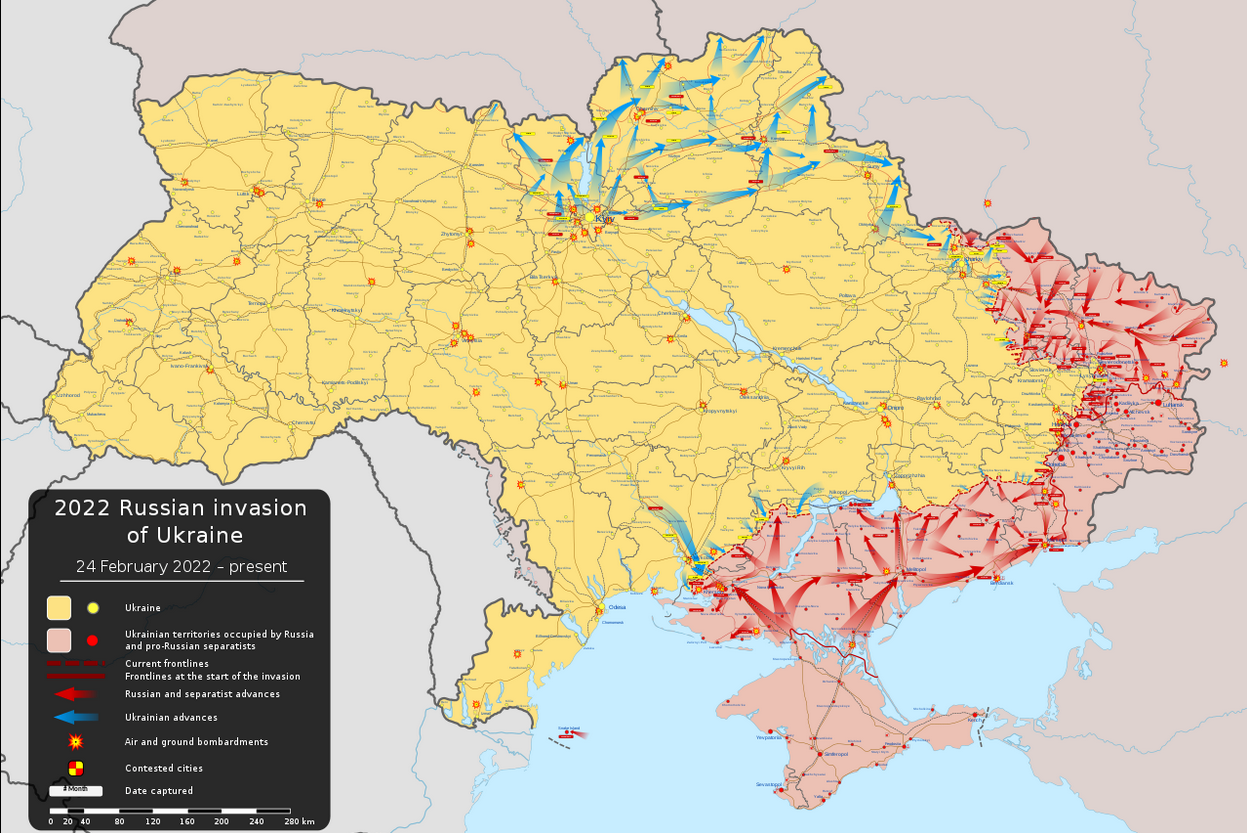
\includegraphics[width=\textwidth,height=\textheight, keepaspectratio]{29june2022ukraine.png}
	\end{figure}
\end{frame}

%same source, screenshotted 16 september but site said it was current as of 14 september
\begin{frame} 
	\frametitle{\LARGE{Conflict Map (14 September 2022)}}
	\begin{figure}[ht!]
		\centering
		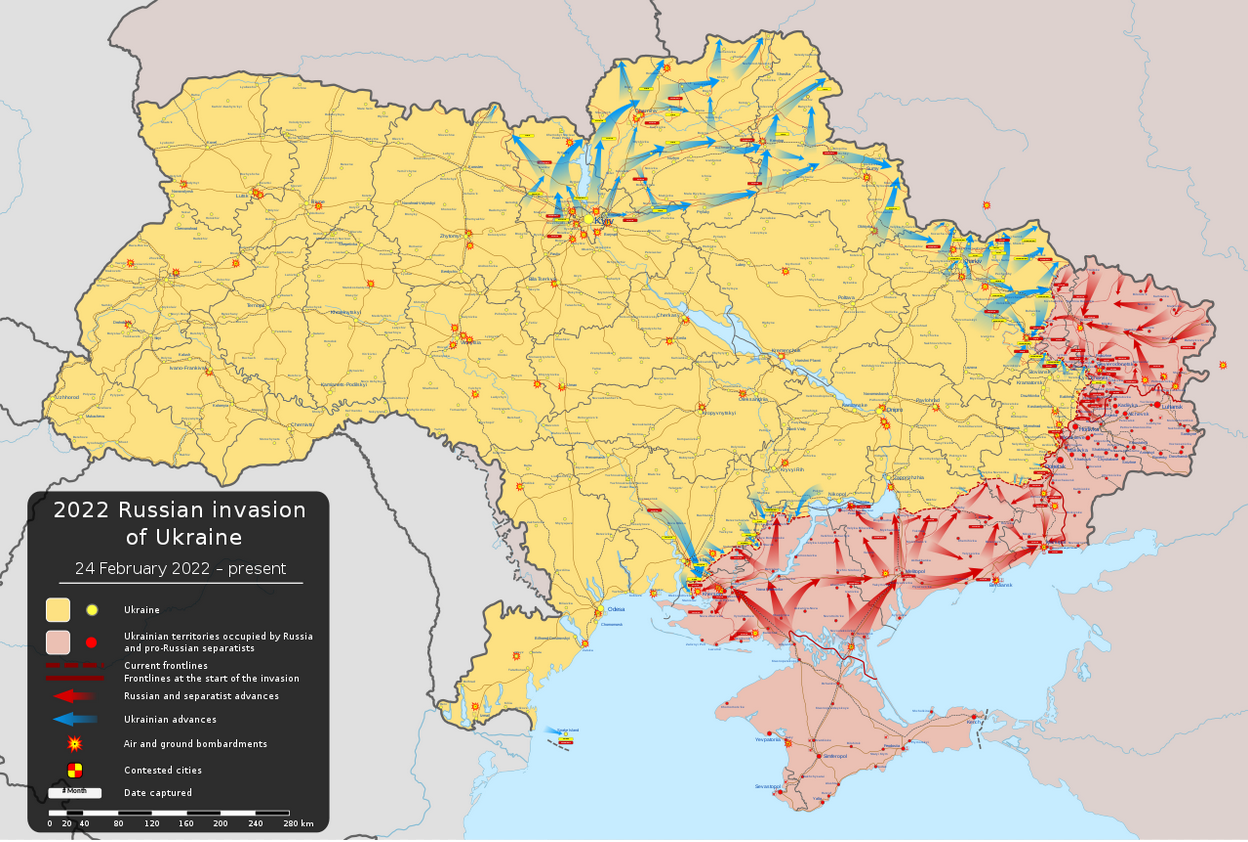
\includegraphics[width=\textwidth,height=\textheight, keepaspectratio]{14sept2022ukraine.png}
	\end{figure}
\end{frame}

%same source, screenshotted 1 july
\begin{frame} 
	\frametitle{\LARGE{Conflict Map (1 July 2023)}}
	\begin{figure}[ht!]
		\centering
		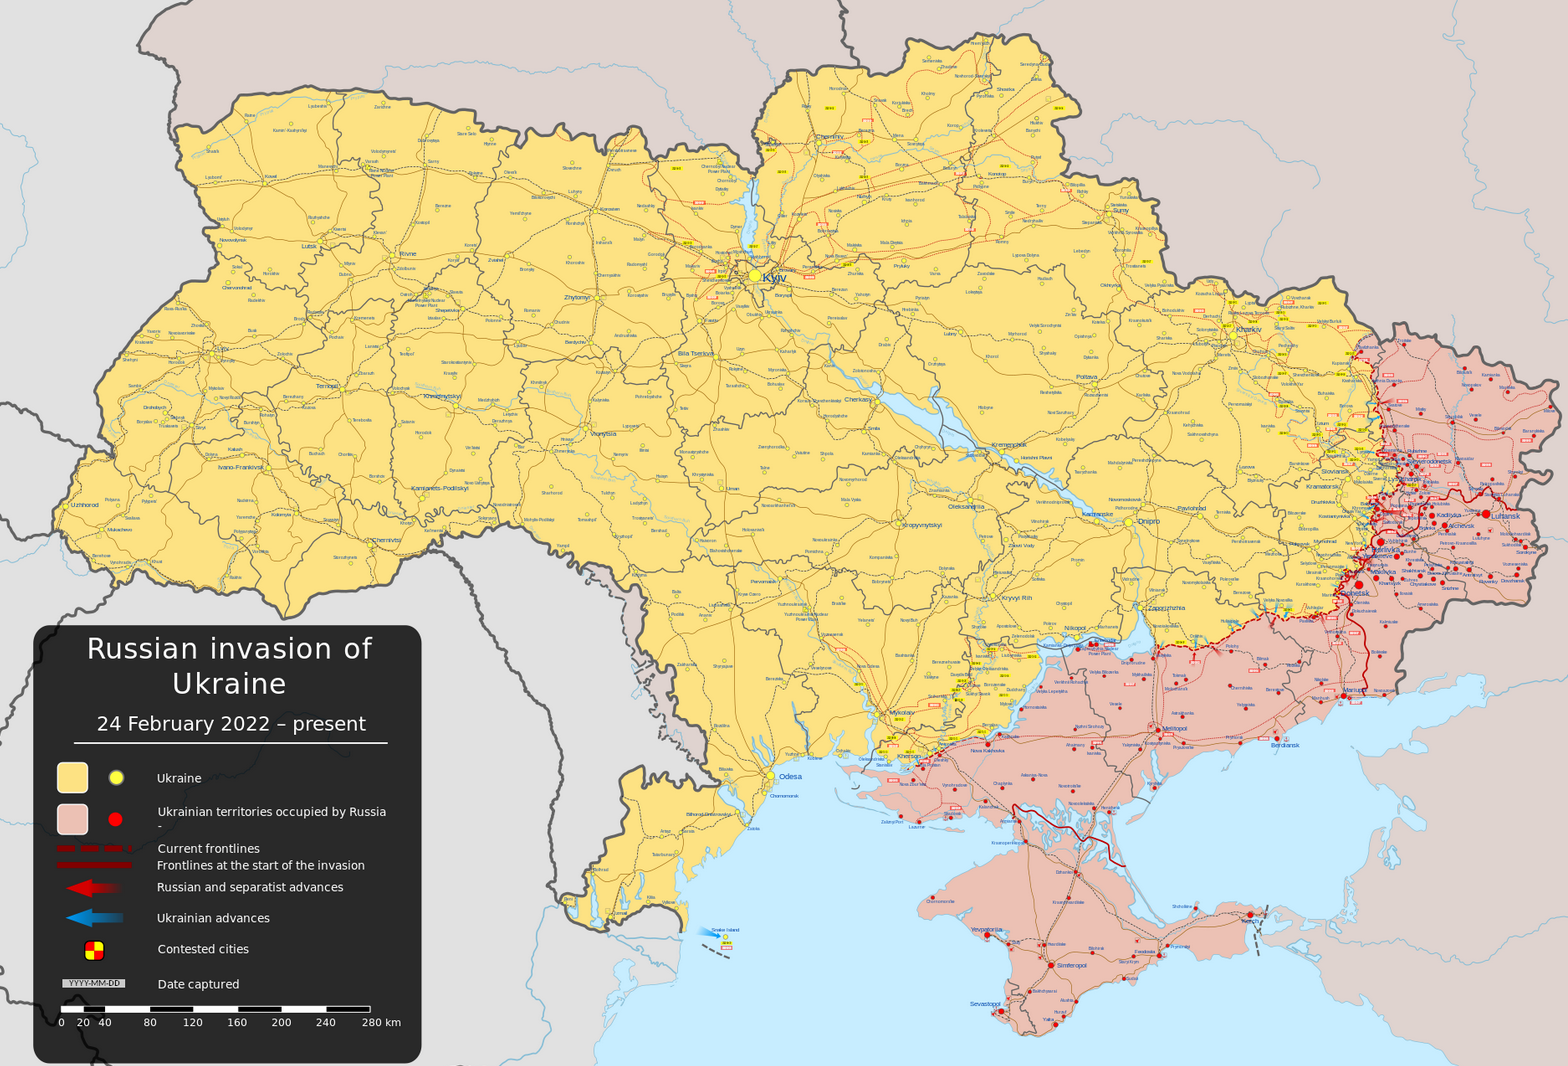
\includegraphics[width=\textwidth,height=\textheight, keepaspectratio]{1july2023ukraine.png}
	\end{figure}
\end{frame}

\begin{frame} 
	\frametitle{\LARGE{Ongoing Costs of War}}
	\begin{itemize}
		\item Costs of war: exact casualty counts \href{https://en.wikipedia.org/wiki/Russian_invasion_of_Ukraine\#Casualties}{vary} but are substantial, and higher than expected by Russian command. \pause
		\item Approx. 8 million refugees have left Ukraine, creating a substantial refugee crisis and strain on neighboring states. \pause
		\item Widespread regional and global economic disruption contributed to global supply chain issues in 2022. \pause
		\item Wide variety of war crimes alleged and committed by Russian forces. \pause
		\item Internal disruption in Russia: Wagner group mutiny and continued uncertainty. \pause
		\item Conflict seems likely to continue.
	\end{itemize}
\end{frame}




\end{document}
